% Frozen Tier 1 protocol for the N83 full-scan / zero-gap canonicalization pair.
% Source of figures/protocol_diagram.pdf; build: pdflatex protocol_diagram.tex
\documentclass[border=6pt]{standalone}
\usepackage{tikz}
\usetikzlibrary{positioning,arrows.meta,decorations.pathreplacing}
\begin{document}
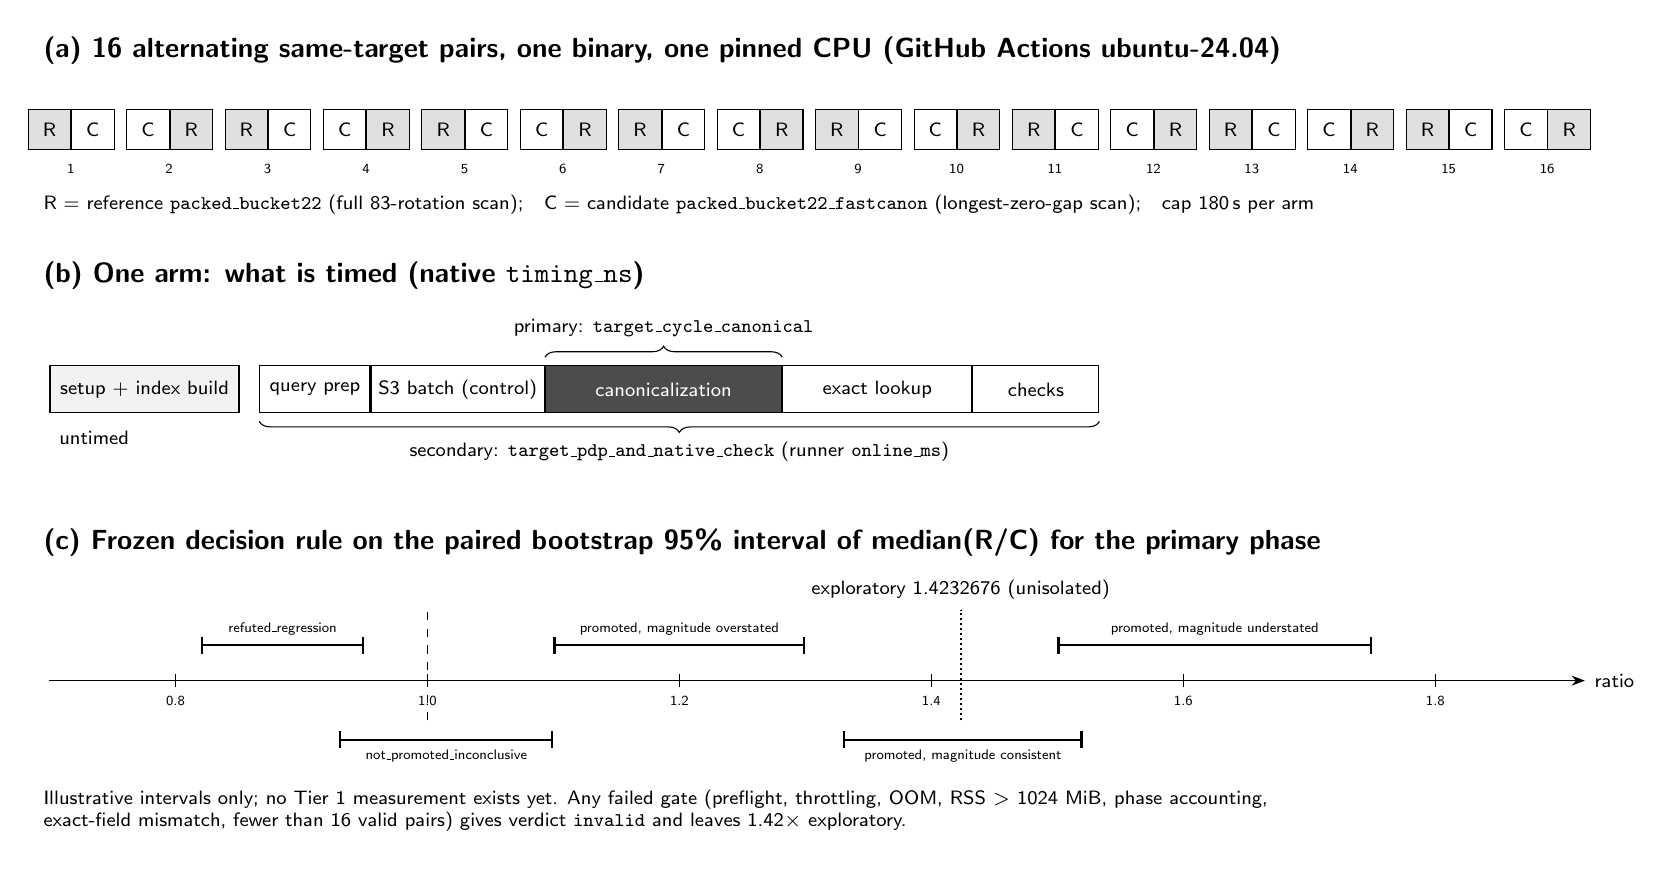
\begin{tikzpicture}[font=\sffamily\small,
  arm/.style={draw, minimum width=5.4mm, minimum height=5mm, inner sep=0pt, font=\sffamily\scriptsize},
  R/.style={arm, fill=gray!25}, C/.style={arm, fill=white},
  phase/.style={draw, minimum height=6mm, inner sep=1pt, font=\sffamily\scriptsize}]
% --- (a) pair schedule
\node[anchor=west, font=\sffamily\bfseries] at (-0.2,1.0) {(a) 16 alternating same-target pairs, one binary, one pinned CPU (GitHub Actions ubuntu-24.04)};
\foreach \i in {0,...,15} {
  \pgfmathsetmacro{\x}{\i*1.25}
  \ifodd\i
    \node[C] at (\x,0) {C}; \node[R] at (\x+0.55,0) {R};
  \else
    \node[R] at (\x,0) {R}; \node[C] at (\x+0.55,0) {C};
  \fi
  \node[font=\sffamily\tiny] at (\x+0.27,-0.5) {\the\numexpr\i+1\relax};
}
\node[anchor=west, font=\sffamily\scriptsize] at (-0.2,-0.95) {R = reference \texttt{packed\_bucket22} (full 83-rotation scan);\quad C = candidate \texttt{packed\_bucket22\_fastcanon} (longest-zero-gap scan);\quad cap 180\,s per arm};
% --- (b) timed interval of one arm
\begin{scope}[yshift=-3.3cm]
\node[anchor=west, font=\sffamily\bfseries] at (-0.2,1.45) {(b) One arm: what is timed (native \texttt{timing\_ns})};
\node[phase, minimum width=2.4cm, fill=gray!10, anchor=west] (setup) at (0,0) {setup + index build};
\node[phase, minimum width=1.4cm, anchor=west, right=0.25 of setup] (q) {query prep};
\node[phase, minimum width=2.2cm, anchor=west, right=0pt of q] (s3) {S3 batch (control)};
\node[phase, minimum width=3.0cm, anchor=west, right=0pt of s3, fill=black!70, text=white] (canon) {canonicalization};
\node[phase, minimum width=2.4cm, anchor=west, right=0pt of canon] (look) {exact lookup};
\node[phase, minimum width=1.6cm, anchor=west, right=0pt of look] (rest) {checks};
\draw[decorate, decoration={brace, amplitude=4pt, mirror}] ([yshift=-1mm]q.south west) -- ([yshift=-1mm]rest.south east)
  node[midway, below=4pt, font=\sffamily\scriptsize] {secondary: \texttt{target\_pdp\_and\_native\_check} (runner \texttt{online\_ms})};
\draw[decorate, decoration={brace, amplitude=4pt}] ([yshift=1mm]canon.north west) -- ([yshift=1mm]canon.north east)
  node[midway, above=4pt, font=\sffamily\scriptsize] {primary: \texttt{target\_cycle\_canonical}};
\node[font=\sffamily\scriptsize, anchor=north west] at (0,-0.4) {untimed};
\end{scope}
% --- (c) decision rule on the paired bootstrap 95% interval of the median ratio R/C
\begin{scope}[yshift=-7.0cm]
\node[anchor=west, font=\sffamily\bfseries] at (-0.2,1.75) {(c) Frozen decision rule on the paired bootstrap 95\% interval of median(R/C) for the primary phase};
\draw[-{Stealth}] (0,0) -- (19.5,0) node[right, font=\sffamily\scriptsize] {ratio};
\foreach \v/\l in {0.8/0.8, 1.0/1.0, 1.2/1.2, 1.4/1.4, 1.6/1.6, 1.8/1.8} {
  \pgfmathsetmacro{\x}{(\v-0.7)*16}
  \draw (\x,0.08) -- (\x,-0.08) node[below, font=\sffamily\tiny] {\l};
}
\pgfmathsetmacro{\one}{(1.0-0.7)*16}
\pgfmathsetmacro{\expl}{(1.4232676-0.7)*16}
\draw[dashed] (\one,-0.5) -- (\one,0.9);
\draw[densely dotted, thick] (\expl,-0.5) -- (\expl,0.9) node[above, font=\sffamily\scriptsize] {exploratory 1.4232676 (unisolated)};
\draw[|-|, thick] ({(0.82-0.7)*16},0.45) -- ({(0.95-0.7)*16},0.45) node[midway, above, font=\sffamily\tiny] {refuted\_regression};
\draw[|-|, thick] ({(0.93-0.7)*16},-0.75) -- ({(1.10-0.7)*16},-0.75) node[midway, below, font=\sffamily\tiny] {not\_promoted\_inconclusive};
\draw[|-|, thick] ({(1.10-0.7)*16},0.45) -- ({(1.30-0.7)*16},0.45) node[midway, above, font=\sffamily\tiny] {promoted, magnitude overstated};
\draw[|-|, thick] ({(1.33-0.7)*16},-0.75) -- ({(1.52-0.7)*16},-0.75) node[midway, below, font=\sffamily\tiny] {promoted, magnitude consistent};
\draw[|-|, thick] ({(1.50-0.7)*16},0.45) -- ({(1.75-0.7)*16},0.45) node[midway, above, font=\sffamily\tiny] {promoted, magnitude understated};
\node[anchor=west, font=\sffamily\scriptsize, align=left] at (-0.2,-1.65) {Illustrative intervals only; no Tier 1 measurement exists yet. Any failed gate (preflight, throttling, OOM, RSS $>$ 1024 MiB, phase accounting,\\
exact-field mismatch, fewer than 16 valid pairs) gives verdict \texttt{invalid} and leaves 1.42$\times$ exploratory.};
\end{scope}
\end{tikzpicture}
\end{document}
